\documentclass[12pt]{article}

\usepackage[a4paper,  top=1.3in, bottom=1.4in, left=1.4in, right=1.5in]{geometry}

\usepackage[utf8]{inputenc}
\usepackage[T1]{fontenc}
\usepackage{amsmath}
\usepackage{amsfonts}
\usepackage{amssymb}


\usepackage{graphicx, float}
\usepackage{adjustbox}
\graphicspath{{images/}}

% \renewcommand{\figurename}{Slika}



\renewcommand{\baselinestretch}{1.2} % Line spacing

% Parskip and parindent
\setlength{\parindent}{0pt} % Begin of paragraph indentation
\setlength{\parskip}{1em} % Paragraph spacing

%--- for references ---------
\usepackage[
    backend=biber,
    style=numeric,
    sorting=none
    ]{biblatex}

\addbibresource{bibliography.bib}
\AtBeginBibliography{\vspace*{10pt}}
%----------------------------

%----------- toc ------------------------
\usepackage{tocloft}
\usepackage{fancyhdr}
% \setlength{\cftbeforesecskip}{0pt} % Adjust the spacing before section entries
% \setlength{\cftbeforesubsecskip}{0pt} % Adjust the spacing before subsection entries
%----------------------------------------

\begin{document}
\pagenumbering{gobble}  % Suppress page numbers initially

% Title Page
\newgeometry{top=1in, bottom=1in, left=1in, right=1in} % New margins for title page
\begin{titlepage}
    \begin{center}
        
        % add your university logo here
        % negative value moves the logo up
        \vspace*{-1in}
        
\includegraphics[width=0.4\textwidth]{raf_logo.png}

        % set font size to 14pt
        \vspace{1in}
        \Large
        \textbf{Review on the topic of}
        
        % set horizontal margin for the title to 1.5in and center it
        \vspace{1in}
        \Huge
        \textbf{Simultaneous localization and mapping (SLAM)}
        
        \vspace{1in}


            \fontsize{17pt}{17pt}\selectfont
            \textbf{Course: Robotics} \\
            \vspace*{1.5in}
            
            \begin{center}
            \normalsize
            \begin{tabular}{p{0.75\textwidth} p{0.5\textwidth}}
                \fontsize{14pt}{18pt}\selectfont   
                \textbf{Advisor:} & 
            
                \fontsize{14pt}{18pt}\selectfont
                \textbf{Student:} \\
                prof. Miloš Jovanović & Vanja Kovinić \\
            \end{tabular}
            \end{center}

            \vspace*{\fill}

            \normalsize
            Belgrade, 2025.


            
        \end{center}
    \end{titlepage}
    \restoregeometry % Restore original margins

    \newpage
    \newgeometry{top=1.3in, bottom=2.2in, left=1.4in, right=1.4in} % New margins for title page

    \tableofcontents

    \newpage
    \clearpage             % Move to a new page
    \pagenumbering{arabic} % Start using Arabic numerals
    \setcounter{page}{1}   % Set the counter to 1
    \section{Introduction to SLAM}
    \subsection{Definition and Problem Statement}
    \textbf{Simultaneous Localization and Mapping (SLAM)} represents one of the fundamental challenges in robotics. At its core, SLAM addresses a deceptively simple question: 
    \\ \textit{How can a mobile robot build a map of an unknown environment while simultaneously determining its own position within that map?} 
    \\ This seemingly straightforward task embodies a classic \textit{"chicken-and-egg"} problem - to create an accurate map, the robot needs to know its precise location,
    but to determine its location, it needs an accurate map.
    \\ The SLAM problem can be formally defined as the process of constructing or updating a map of an unknown environment while keeping track of an agent's location within it. 
    Mathematically, SLAM estimates both the trajectory of the robot ($X_{1} = {x_1, x_2, \ldots, x_t}$) and the map of the environment ($M$) given the observations ($Z_{1}$) and control inputs ($U_{1}$):
    \[p(X_{1}, M \mid Z_{1}, U_{1})\]
    This joint probability distribution encapsulates the inherent uncertainty in both the robot's position and the environmental map, recognizing that both must be estimated simultaneously.

    \newpage

    The technical challenges of SLAM extend beyond this core problem. Real-world implementations must contend with:
    \begin{enumerate}
        \item \textbf{Sensor limitations}: All sensors provide imperfect measurements with noise, limited range, and potential occlusions.
        \item \textbf{Data association}: Determining whether sensor observations correspond to previously observed landmarks or represent new features.
        \item \textbf{Loop closure}: Recognizing when the robot has returned to a previously visited location, allowing for correction of accumulated errors.
        \item \textbf{Computational efficiency}: Balancing accuracy with real-time performance requirements, especially on platforms with limited computing resources.
        \item \textbf{Environmental dynamics}: Managing changes in the environment, such as moving objects or changing conditions.
    \end{enumerate}

    \begin{figure}[h!]
        \centering
        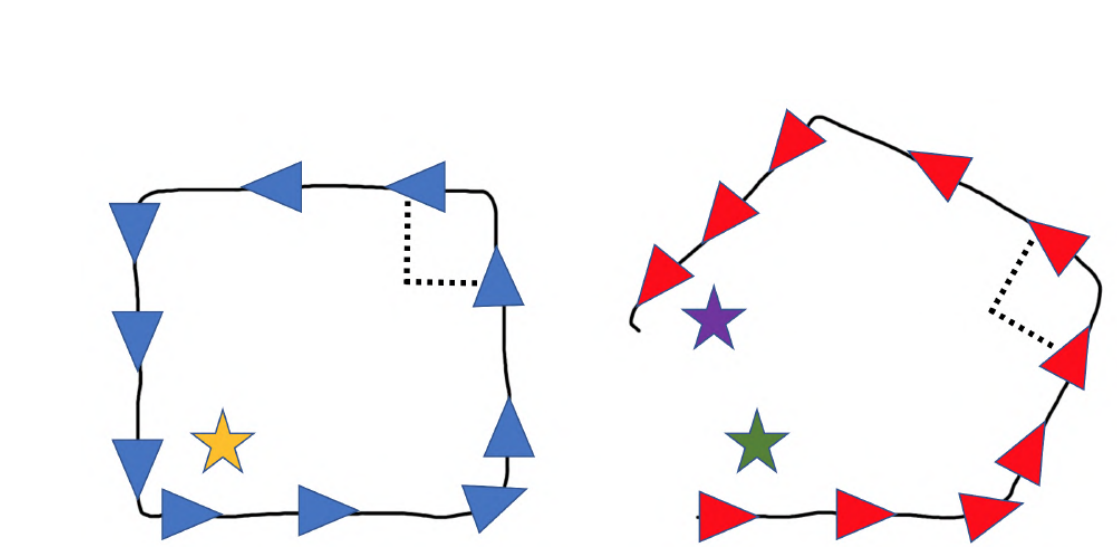
\includegraphics[width=0.8\textwidth]{loop_closure.png}
        \caption{The diagram shows loop closure in robot mapping. When a feature is recognized again (left), a constraint is added to correct the robot's trajectory. 
        If the feature is not recognized (right), errors in the estimated path remain uncorrected. \cite{loop_closure_img}}
        \label{fig:loop_closure}
    \end{figure}

    A successful SLAM system must integrate sensor data over time while accounting for uncertainties and constraints to produce a consistent representation of both the robot's path 
    and the surrounding environment.

    \newpage

    \subsection{Historical Context and Importance in Robotics}
    The development of SLAM techniques represents a crucial milestone in the evolution of autonomous robotics. Before SLAM, robots relied on pre-built maps or simple reactive behaviors, 
    severely limiting their autonomy and usefulness in unknown environments.
    The conceptual foundations of SLAM emerged in the 1980s through seminal work by researchers such as Hugh Durrant-Whyte and John J. Leonard \cite{seminal_paper}, who recognized 
    to the statistical correlations between landmarks in a map. However, the term "SLAM" itself was not coined until the early 1990s.

    The historical progression of SLAM research can be divided into several key phases:

    \begin{enumerate}
        \item \textbf{Early probabilistic approaches (1990s)}: The initial formulation of SLAM using Extended Kalman Filters (EKF) provided the mathematical framework for 
        handling uncertainty in both robot motion and sensing \cite{early_probabilistic_approaches}. These approaches were limited by computational complexity that scaled quadratically with the number of landmarks.
        \item \textbf{Particle filter methods (early 2000s)}: FastSLAM \cite{fast_slam} and other particle filter approaches offered improved performance for nonlinear systems and 
        non-Gaussian noise, enabling more robust implementations.
        \item \textbf{Graph-based optimization (mid-2000s)}: The formulation of SLAM as a sparse graph optimization problem led to more efficient solutions 
        that could handle larger environments and longer trajectories.
        \item \textbf{Visual SLAM systems (2007-2015)}: The incorporation of camera data enabled systems like MonoSLAM \cite{monoslam}, PTAM, and ORB-SLAM \cite{orb_slam}, which could operate 
        using only visual information without specialized ranging sensors.
        \newpage
        \item \textbf{Learning-based approaches (2015-present)}: The integration of deep learning methods has pushed the boundaries of SLAM performance, particularly 
        in feature extraction, depth estimation, and semantic understanding.
    \end{enumerate}

    The introduction of SLAM algorithms effectively gave robots a spatial intelligence - the ability to interpret, map, and navigate previously unseen environments without human guidance.
    Some of the most notable applications of SLAM include:
    \begin{itemize}
        \item \textbf{Autonomous vehicles}: Tesla's FSD system and Waymo's autonomous taxis implement sophisticated SLAM variants that fuse visual data with other sensor modalities. 
        Their ability to navigate complex urban environments relies not just on GPS (which fails in tunnels or urban canyons) but on real-time environmental mapping at centimeter-level precision.
        \item \textbf{Disaster response}: After the Fukushima nuclear disaster, robots equipped with RGBD-SLAM systems entered radiation-contaminated zones inaccessible to humans,
        creating 3D maps that enabled remote assessment of structural damage without endangering human lives \cite{fukushima_disaster}.
        \item \textbf{Domestic robotics}: The evolution of cleaning robots from random bouncers like early Roombas to the systematic path-planners seen in Roborock S7 models 
        illustrates how SLAM transformed consumer robotics from novelties into genuinely useful tools that can efficiently cover complex home layouts.
        \item \textbf{Mixed reality}: Apple's ARKit and Microsoft's HoloLens use visual-inertial SLAM to maintain stable positioning of virtual objects in the physical world, enabling 
        applications from surgical training to architectural visualization that rely on precise spatial registration.
    \end{itemize}

    \begin{figure}[h!]
        \centering
        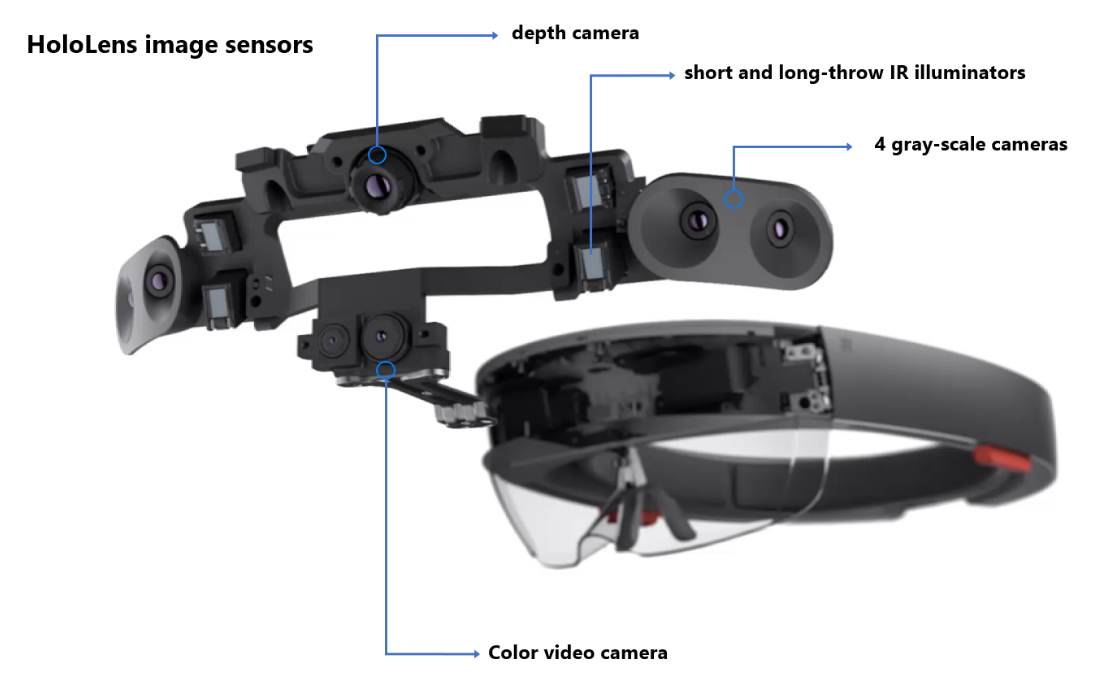
\includegraphics[width=0.7\textwidth]{mcsft_hololens.png}
        \caption{Microsoft HoloLens uses SLAM by fusing data from cameras, depth sensors, and IMUs to simultaneously track the headset’s position and map the environment. 
        This enables accurate placement of virtual objects in the real world for stable and immersive augmented reality experiences.}
        \label{fig:mcsft_hololens}
    \end{figure}


    \section{Fundamental Challenges in SLAM}

    \subsection{The Chicken-and-Egg Problem}
    
    The core paradox of SLAM is deceptively simple: to build an accurate map, a robot needs to know its precise location, but to determine its location accurately, it needs a reliable map. 
    This interdependence creates the \textit{"chicken-and-egg problem"} of SLAM.
    
    Consider a robot entering an unknown room. To map the room accurately, it must know exactly how far it has moved since entering. However, small errors in wheel encoders, IMU drift, or visual
    tracking cause position uncertainty to grow. 
    
    Without external references, these errors accumulate - a phenomenon known as "dead reckoning drift". After moving just a few meters, the robot's position estimate might be off by several centimeters, 
    causing all mapped features to be misplaced.
    This circular dependency manifests in two critical ways:
    
    First, position estimation errors directly propagate into the map. Imagine a robot that turns a corner and incorrectly estimates its rotation by 2 degrees. This small angular error will cause all subsequent 
    wall measurements to be tilted, creating a distorted map. When the robot later tries to localize using this faulty map, its position estimates become increasingly unreliable.

    Second, without correction mechanisms, uncertainty grows unbounded over time. A robot navigating a long corridor might start with centimeter-level position accuracy, but after traveling 20 meters, drift might increase 
    to decimeter-level errors. This uncertainty expansion makes long-term SLAM inherently unstable without additional constraints.
    
    The probabilistic SLAM framework addresses this by maintaining a joint distribution over both the robot's trajectory and map features:
    \[p(x_t, m | z_{1}, u_{1}, x_0)\]

    Where $x_t$ is the robot's pose at time $t$, $m$ is the map, $z_{1}$ are sensor observations, $u_{1}$ are control inputs, and $x_0$ is the initial pose.
    This formulation acknowledges that robot positions and landmark locations are correlated random variables that must be estimated together, not independently. The correlation is intuitive: 
    if we learn that a landmark is farther to the right than previously estimated, the robot was likely more to the left than we thought.
    Classic SLAM approaches handle this correlation through:

    \begin{itemize}
        \item Maintaining the full covariance matrix between pose and map variables in EKF-SLAM \cite{ekf_slam}
        \item Sampling multiple potential trajectories in particle filter approaches like FastSLAM \cite{fast_slam}
        \item Building a graph of spatial constraints that can be jointly optimized in modern graph-based SLAM
    \end{itemize}

    \newpage
    While the chicken-and-egg problem cannot be eliminated completely, these mathematical frameworks manage it by simultaneously optimizing for consistent mapping and localization, effectively distributing errors 
    throughout the system rather than allowing them to accumulate unconstrained.    
    
    \subsection{Sensor Limitations and Environmental Factors}
    
    Every SLAM system must contend with the limitations of its perception hardware and challenging environmental conditions:
    
    \textbf{LiDAR Sensors} struggle with reflective or transparent surfaces, have limited range, and suffer from motion distortion during scanning.
    
    \textbf{RGB Cameras} face scale ambiguity (in monocular setups), illumination sensitivity, difficulty with texture-less regions, and degraded performance from motion blur.
    
    \textbf{Depth Cameras} have shorter range than LiDAR, perform poorly in bright sunlight, and produce noisy measurements at object edges.
    
    \textbf{Inertial Measurement Units} accumulate drift through integration and suffer from changing bias and noise.
    
    Beyond sensor limitations, environmental factors pose additional challenges:
    
    \textbf{Perceptual Aliasing:} Repetitive environments (office corridors, parking structures) create ambiguity as different locations appear identical.
    
    \textbf{Featureless Environments:} Spaces lacking distinctive features provide insufficient information for reliable localization.
    
    \textbf{Dynamic Objects:} Moving elements like people or rearranged furniture violate the static world assumption in many SLAM formulations.
    
    \textbf{Temporal Changes:} Outdoor environments undergo appearance changes with seasons, weather, and time of day.
    
    Successful SLAM implementations address these challenges through sensor fusion, robust feature selection, outlier rejection, and specialized algorithms for dynamic environments.
    
    \subsection{Loop Closure and Data Association}
    Loop closure (recognizing when a robot has returned to a previously visited location) represents perhaps the most powerful constraint in SLAM systems. 
    Without loop closure, errors accumulate unbounded over time, resulting in inconsistent maps and increasingly inaccurate localization. 
    When properly detected and incorporated, loop closures can dramatically improve map consistency by distributing accumulated errors throughout the trajectory.
    
    To understand the significance of loop closure, consider a robot exploring an office building. Starting from the lobby, it navigates through corridors, accumulating small errors in its position 
    estimate. After circling back to the lobby 15 minutes later, its estimated position might be off by several meters from its actual position. Without recognizing the lobby, the robot would produce a map 
    with disconnected segments and potentially overlapping walls. Upon detecting that it has returned to the lobby, the system can "close the loop," triggering a global optimization that realigns the 
    entire trajectory and map.

    \begin{figure}[h!]
        \centering
        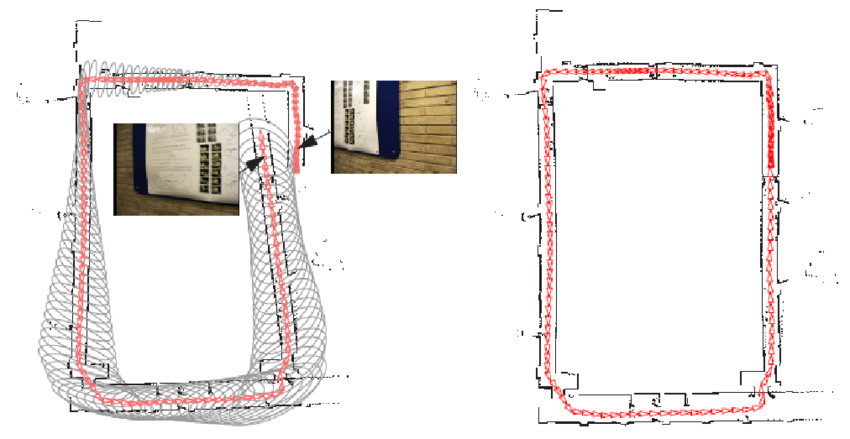
\includegraphics[width=0.7\textwidth]{loop_closure_2.png}
        \caption{Left image: Robot's path before loop closure, showing growing uncertainty (gray ellipses) and misalignment at the loop point. Camera views used for matching are inset. 
                Right image: Corrected map after loop closure, with aligned positions and reduced errors. \cite{loop_closure_2_img}}
        \label{fig:loop_closure_2}
    \end{figure}

    \newpage

    Loop closure detection faces several significant challenges:

    \textbf{Viewpoint variation}: The robot may approach the same location from a completely different direction. A corridor observed initially from north to south looks substantially different when viewed from south to north.
    
    \textbf{Perceptual aliasing}: Many environments contain similar-looking areas. In a hospital, multiple identical-looking corridors can trigger false loop closures that catastrophically distort the map.
    
    \textbf{Accumulated pose error}: By the time the robot returns to a known location, its position uncertainty may be so large that the expected and actual observations have minimal overlap.
    
    \textbf{Appearance changes}: Lighting conditions, moved objects, seasonal variations, and human activities can dramatically alter how the same location appears at different times.


    \newpage

    Modern loop closure approaches implement multi-stage processing:

    \begin{itemize}
        \item \textbf{Place recognition}: Identifying candidate locations, often using appearance-based methods such as visual bag-of-words models (DBoW), sequence-to-sequence matching, or learned embedding spaces that map 
        similar locations close together regardless of viewpoint or illumination.
        \item \textbf{Geometric verification}: Confirming candidates by establishing geometric consistency through feature matching and transformation estimation.
        \item \textbf{Global consistency checking}: Validating that the proposed loop closure is consistent with the existing map and trajectory, sometimes using techniques like RRR (Realizing, Reversing, Recovering) to reject outliers.
        \item \textbf{Graph optimization}: Incorporating verified loop closures as constraints in a pose graph that is globally optimized to distribute errors throughout the trajectory.
    \end{itemize}

    Loop closure is intimately connected with data association - the process of matching current observations with previously established map elements. While loop closure operates at the 
    level of places, data association functions across multiple levels. It enables low-level feature matching between consecutive frames for visual odometry, facilitates landmark 
    identification by associating observed features with mapped landmarks, and supports object recognition by identifying and tracking objects across multiple observations.

    While structured, static environments are reasonably well-handled by current algorithms, dynamic, changing, or visually ambiguous environments continue to pose significant difficulties that drive ongoing research.

    \section{Classical Approaches to SLAM}

    \subsection{Filter-Based Methods}
    
    Filter-based methods dominated early SLAM research, providing principled approaches to handling the inherent uncertainties in robot motion and sensing. These methods recursively estimate the posterior probability distribution over 
    robot poses and map features as new observations arrive.
    
    \textbf{Extended Kalman Filter SLAM (EKF-SLAM)} was the first widely adopted approach to SLAM. Introduced in the early 1990s, EKF-SLAM represents the joint state of the robot and map features with a multivariate Gaussian distribution, 
    maintaining both mean estimates and their uncertainty through a covariance matrix.
    
    The EKF-SLAM algorithm operates in two phases:
    \begin{itemize}
        \item \textbf{Prediction step}: Updates the state estimate based on robot motion, typically increasing uncertainty
        \item \textbf{Correction step}: Incorporates sensor measurements to update both the state estimate and reduce uncertainty
    \end{itemize}

    \begin{figure}[h!]
        \centering
        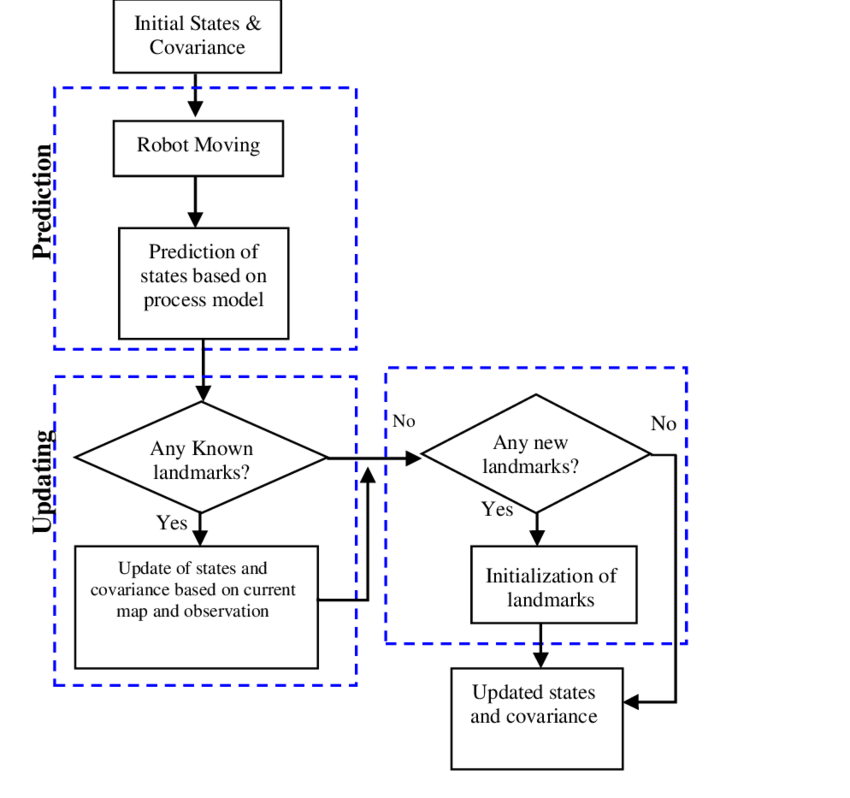
\includegraphics[width=0.7\textwidth]{D-EKF-SLAM-operation.png}
        \caption{This flowchart shows the EKF-SLAM algorithm process. Starting with initial states and covariance, it follows a prediction phase when the robot moves, 
        then branches into an update phase that either updates existing landmarks or initializes new ones, ultimately producing updated states and covariance. \cite{ekf_slam_img}}
        \label{fig:D-EKF-SLAM-operation}
    \end{figure}
    
    The mathematical formulation involves:
    \begin{itemize}
        \item State vector $\mathbf{x} = [\mathbf{x}_r, \mathbf{m}_1, \mathbf{m}_2, ..., \mathbf{m}_n]^T$ combining robot pose $\mathbf{x}_r$ and map features $\mathbf{m}_i$
        \item Covariance matrix $\mathbf{P}$ representing uncertainty in the state estimate and correlations between variables
        \item Nonlinear motion model $\mathbf{f}(\mathbf{x}, \mathbf{u})$ with control input $\mathbf{u}$
        \item Nonlinear observation model $\mathbf{h}(\mathbf{x})$ relating state to expected measurements
    \end{itemize}
    
    EKF-SLAM handles the chicken-and-egg problem by explicitly maintaining correlations between the robot pose and map features. When the robot observes a landmark, the uncertainty in both the robot's 
    position and the landmark's position becomes correlated—improving the estimate of one improves the estimate of the other.
    
    However, EKF-SLAM suffers from significant limitations:
    \begin{itemize}
        \item $O(n^2)$ computational complexity with $n$ landmarks, making it unsuitable for large-scale environments
        \item Linearization errors from the extended Kalman filter that can cause inconsistency and divergence
        \item Difficulty handling multi-modal distributions and ambiguous data associations
        \item Sensitivity to outliers in sensor measurements
    \end{itemize}
    
    \textbf{Particle Filter SLAM} addresses some EKF-SLAM limitations by representing the posterior distribution with a set of weighted samples (particles) rather than a single Gaussian. The most influential 
    particle filter approach, FastSLAM, introduced by Montemerlo et al. in 2002 \cite{fast_slam}, uses a Rao-Blackwellized particle filter that:
    \begin{itemize}
        \item Factors the SLAM posterior into robot trajectory and map features conditioned on trajectory
        \item Represents the robot trajectory distribution with particles
        \item Represents map feature estimates with compact EKFs, one per particle
    \end{itemize}
    
    This factorization leverages a key insight: conditioned on the robot trajectory, map features are independent. The FastSLAM algorithm:
    \begin{itemize}
        \item Maintains multiple trajectory hypotheses through particles
        \item Updates individual map features efficiently with separate EKFs
        \item Naturally handles multi-modal distributions and ambiguous data associations
        \item Resamples particles based on observation likelihood, removing unlikely trajectories
    \end{itemize}

    \newpage
    \begin{figure}[h!]
        \centering
        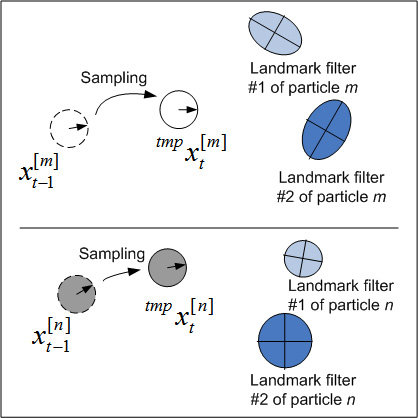
\includegraphics[width=0.7\textwidth]{fast_slam_img.png}
        \caption{This diagram shows the FastSLAM particle filter process. Two particles (m and n) are sampled from previous to temporary states. Particles represent different possible robot pose hypotheses. 
        Each particle maintains separate uncertainty estimates for two landmarks, shown as ellipses - larger ellipses indicate greater positional uncertainty. 
        Light blue ellipses represent landmark filter \#1, while darker blue ellipses represent landmark filter \#2, with the uncertainty patterns varying between particles. \cite{fast_slam_img}}
        \label{fig:fast_slam_img}
    \end{figure}
    
    FastSLAM achieves $O(M \log N)$ complexity for $M$ particles and $N$ landmarks, allowing it to scale better than EKF-SLAM to larger environments.
    
    Despite these advantages, particle filter approaches have their own limitations:
    \begin{itemize}
        \item Particle depletion in high-dimensional spaces
        \item Difficulty representing long trajectories efficiently
        \item Computational constraints on the number of particles
        \item Need for resampling, which can cause loss of diversity
    \end{itemize}
    
    Filter-based methods laid the groundwork for understanding SLAM as a probabilistic estimation problem, but their limitations in handling large-scale environments eventually 
    led to the development of more efficient optimization-based approaches.
    
    \subsection{Graph-Based Optimization}
    
    Graph-based optimization has become the dominant paradigm in modern SLAM systems, offering superior scalability and accuracy compared to filter-based methods. 
    Rather than recursively updating a state estimate, graph-based SLAM formulates the problem as finding the configuration of robot poses and map features that best explains all observations.
    
    The core idea is to represent SLAM as a sparse graph where:
    \begin{itemize}
        \item \textbf{Nodes} represent robot poses and map features
        \item \textbf{Edges} represent constraints from odometry measurements and landmark observations
    \end{itemize}
    
    This approach was pioneered by Lu and Milios in the 1990s but became practical only in the 2000s with the development of efficient optimization techniques. 
    The graph-based formulation transforms SLAM into a nonlinear least squares problem, finding the configuration of nodes that minimizes the sum of squared errors introduced by the constraints.
    
    Mathematically, we aim to find the state vector $\mathbf{x}$ that minimizes:
    
    $$\mathbf{x}^* = \arg\min_{\mathbf{x}} \sum_{i,j} \rho(\mathbf{e}_{ij}^T \mathbf{\Omega}_{ij} \mathbf{e}_{ij})$$
    
    Where:
    \begin{itemize}
        \item $\mathbf{e}_{ij}$ is the error between predicted and measured relative poses or observations
        \item $\mathbf{\Omega}_{ij}$ is the information matrix (inverse covariance) representing constraint certainty
        \item $\rho$ is a robust cost function that reduces the influence of outliers
    \end{itemize}
    
    Key advantages of graph-based SLAM include:
    \begin{itemize}
        \item \textbf{Scalability}: Sparse graph structure enables efficient optimization even for large environments
        \item \textbf{Global consistency}: Optimizes all constraints simultaneously instead of sequential filtering
        \item \textbf{Loop closure integration}: Naturally incorporates loop closures as additional constraints
        \item \textbf{Incremental operation}: Can update the solution efficiently as new information arrives
    \end{itemize}
    
    Graph-based SLAM also integrates well with both traditional and learning-based front-ends that extract constraints from sensor data. 
    The separation of front-end (data association and constraint extraction) from back-end (optimization) has enabled modular system design and focused innovation in each component.
    
    \newpage
    While graph-based optimization overcomes many limitations of filter-based methods, challenges remain:
    \begin{itemize}
        \item \textbf{Initialization sensitivity}: Performance depends on good initial values for optimization
        \item \textbf{Outlier robustness}: False constraints can significantly distort the solution
        \item \textbf{Parameter tuning}: Requires careful selection of robust cost functions and optimization parameters
    \end{itemize}
    
    Nevertheless, graph-based optimization has proven remarkably successful, becoming the foundation for most state-of-the-art SLAM systems in the last decade.
    
    \begin{figure}[h!]
        \centering
        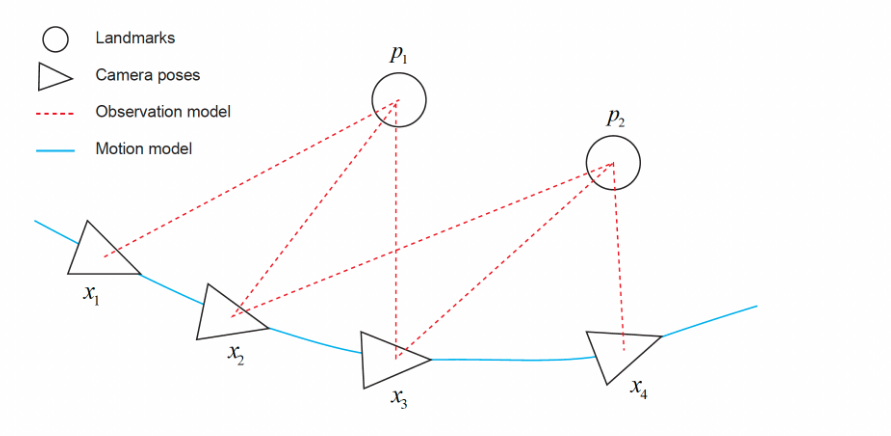
\includegraphics[width=1.1\textwidth]{graph_based_optimization.png}
        \caption{An example of the graph optimization. \cite{graph_optimization_img}}
        \label{fig:graph_based_optimization}
    \end{figure}

    \newpage
    \subsection{Traditional Visual SLAM Systems}
    Visual SLAM systems use cameras as their primary sensing modality, offering rich environmental information at relatively low cost. Three main approaches have emerged in traditional visual SLAM:
    
    \textbf{1. Feature-based methods} detect and track distinctive points across frames, using them as landmarks. These systems typically operate through feature detection, description, matching, 
    motion estimation, and bundle adjustment to optimize camera poses and feature positions. Key innovations include parallel tracking and mapping threads and keyframe-based representations.
    
    \textbf{2. Direct methods} operate on image intensity values without extracting features, potentially using all pixels rather than sparse points. These approaches minimize photometric error rather than 
    geometric reprojection error and can work in less textured environments where feature detection might fail.
    
    \textbf{3. Hybrid approaches} combine elements of both feature-based and direct methods for increased robustness and efficiency.
    Traditional visual SLAM systems face several challenges: scale ambiguity in monocular setups, difficult initialization, sensitivity to dynamic objects and illumination changes, and poor performance in textureless regions. 
    Many systems address these limitations by incorporating additional sensing modalities like stereo cameras, RGB-D sensors, or IMUs.
    Despite impressive performance in controlled environments, traditional visual SLAM approaches still struggle with perceptual aliasing, long-term operation in changing environments, and semantic 
    understanding—limitations that have motivated the integration of learning-based methods.

    \newpage

    \section{Deep Learning in Modern SLAM}

    Deep learning has revolutionized numerous aspects of SLAM systems, addressing many limitations of traditional approaches while introducing new capabilities. 
    Rather than completely replacing geometric methods, learning-based components typically enhance SLAM pipelines by leveraging data-driven insights where classical algorithms struggle.
    
    \subsection{Learned Features vs. Handcrafted Features}
    
    Traditional SLAM systems rely on handcrafted feature detectors and descriptors like SIFT \cite{sift}, SURF \cite{surf}, and ORB \cite{orb_slam}, which were designed based on human intuition about what makes points distinctive and matchable. 
    While effective in many scenarios, these features have inherent limitations:
    
    \begin{itemize}
        \item Poor performance under challenging conditions (illumination changes, motion blur)
        \item Limited robustness to viewpoint variations
        \item Difficulty in textureless or repetitive environments
        \item Inability to adapt to specific domains without manual tuning
    \end{itemize}
    
    Deep learning has transformed feature extraction through learned alternatives that outperform traditional methods in robustness and accuracy. 
    These approaches typically use convolutional neural networks (CNNs) trained on large datasets of image pairs with known correspondences.
    
    \newpage
    Learned feature detectors identify keypoints that are:
    \begin{itemize}
        \item Repeatable across different views and conditions
        \item Distinctive enough for reliable matching
        \item Accurately localizable in the image
    \end{itemize}
    
    Key advantages of learned features include:
    \begin{itemize}
        \item \textbf{Adaptability}: Can be trained for specific environments or conditions
        \item \textbf{Context awareness}: Consider wider image context beyond local patches
        \item \textbf{Task optimization}: Can be trained specifically for SLAM performance metrics
        \item \textbf{Robustness}: Better handling of challenging conditions than handcrafted features
    \end{itemize}
    
    Many modern systems adopt a hybrid approach, using learned features for challenging situations while maintaining handcrafted features for computational efficiency in standard conditions. 
    This combination leverages the strengths of both paradigms: the proven reliability of geometric methods and the adaptability of learning-based approaches.
    
    \newpage
    \subsection{End-to-End SLAM Architectures}
    
    End-to-end SLAM architectures represent the most ambitious application of deep learning to SLAM, aiming to replace traditional modular pipelines with neural networks that directly map 
    sensor inputs to pose estimates and map representations. These systems attempt to learn the entire SLAM process through data rather than explicit geometric modeling.
    
    Unlike traditional SLAM systems that consist of clearly defined components (feature extraction, matching, pose estimation, mapping, loop closure), end-to-end approaches blur these boundaries, 
    allowing the network to discover its own internal representations and processing steps.
    
    The spectrum of end-to-end SLAM includes:
    
    \textbf{Pose Regression Networks} predict camera poses directly from images or image sequences. While conceptually simple, these approaches often struggle with generalization to new environments and accumulate drift over time, 
    limiting their applicability to short trajectories.
    
    \textbf{Deep Visual Odometry} systems use CNNs or recurrent neural networks (RNNs) to estimate frame-to-frame motion, sometimes incorporating geometric constraints. DeepVO \cite{deepvo} represents early example 
    that demonstrated the potential of learned odometry while highlighting the challenge of preventing drift.
    
    \textbf{Learning-based SLAM Frameworks} integrate deep networks while maintaining some classical components. MapNet \cite{mapnet} combines absolute pose regression with relative pose constraints, while CNN-SLAM \cite{cnnslam} 
    and CodeSLAM \cite{codeslam} use learned components within a traditional SLAM framework.
    
    \textbf{Memory-Augmented Networks} address the mapping aspect by incorporating explicit memory mechanisms that store and retrieve spatial information. Neural SLAM architectures use differentiable memory structures 
    that function similarly to occupancy grids or feature maps, allowing end-to-end training while maintaining interpretable map representations.
    
    
    \newpage
    \begin{figure}[h!]
        \centering
        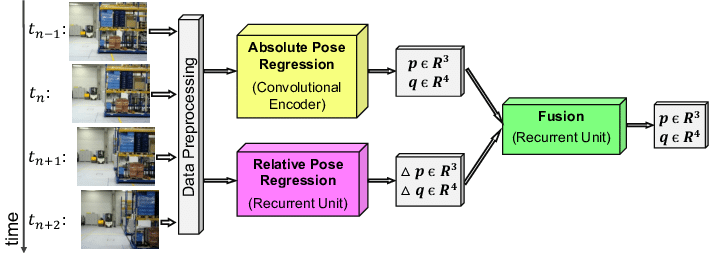
\includegraphics[width=1.0\textwidth]{pose_regression.png}
        \caption{An example of pose regression neural network. \cite{pose_regression_img}}
        \label{fig:pose_regression}
    \end{figure}

    Key challenges in end-to-end SLAM include:
    
    \begin{itemize}
        \item \textbf{Generalization}: Networks trained in specific environments often perform poorly in new settings
        \item \textbf{Data Requirements}: Acquiring sufficient training data with ground truth poses and maps is difficult
        \item \textbf{Interpretability}: Black-box models make debugging and performance guarantees challenging
        \item \textbf{Computational Efficiency}: Deep networks typically require significant computational resources
        \item \textbf{Consistency}: Ensuring global map consistency without explicit loop closure is difficult
    \end{itemize}
    
    Despite these challenges, end-to-end approaches offer intriguing benefits:
    
    \begin{itemize}
        \item \textbf{Adaptability}: Can potentially learn to handle conditions that challenge geometric methods
        \item \textbf{Integration of Semantic Information}: Naturally incorporate object recognition and scene understanding
        \item \textbf{Multimodal Fusion}: Can learn optimal ways to combine different sensor inputs
        \item \textbf{Uncertainty Representation}: Some architectures naturally represent uncertain estimates
    \end{itemize}
    
    Currently, end-to-end SLAM systems have not yet surpassed the best modular approaches in general settings. However, they show particular promise in specific scenarios where geometric assumptions break down, such as 
    highly dynamic environments or scenes with significant non-rigid elements.
    
    \subsection{Neural Implicit Representations for Mapping}
    
    Neural implicit representations have emerged as a powerful alternative to traditional mapping techniques in SLAM. Unlike explicit representations such as point clouds, voxel grids, or mesh surfaces, implicit representations 
    define the environment as a continuous function that maps spatial coordinates to properties like occupancy, signed distance to surfaces, or appearance.
    
    In the context of SLAM, neural networks parameterize these functions, typically as multi-layer perceptrons (MLPs) that take 3D coordinates as input and output properties at those locations. This approach offers several compelling advantages:
    
    \begin{itemize}
        \item \textbf{Continuous Representation}: No discretization artifacts or resolution limitations
        \item \textbf{Memory Efficiency}: Complex scenes represented by network parameters rather than explicit storage
        \item \textbf{Differentiability}: Enables gradient-based optimization and integration with learning pipelines
        \item \textbf{Regularization}: Networks naturally interpolate between observations and regularize noisy data
    \end{itemize}
    
    Several types of neural implicit representations have been applied to SLAM:
    
    \textbf{Neural Radiance Fields (NeRF)} encode both geometry and appearance, representing scenes as continuous volumetric fields. Originally developed for novel view synthesis from static images \cite{nerf_paper}, NeRF has been adapted for SLAM in 
    systems like iNeRF \cite{inerf}, which inverts the rendering process to estimate camera poses, and NICE-SLAM \cite{nice-slam}, which builds NeRF representations incrementally from RGB-D sequences.
    
    \begin{figure}[h!]
        \centering
        \makebox[\textwidth][c]{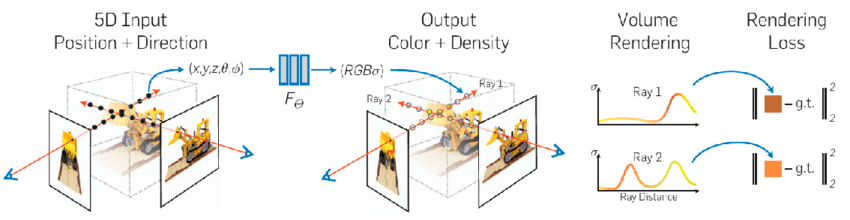
\includegraphics[width=1.1\textwidth]{nerf.png}}
        \caption{This figure illustrates the NeRF pipeline. The left shows 5D input coordinates $(x,y,z,\theta,\phi)$ feeding into a neural network $F_\theta$. 
        The network outputs color and density values $(RGB,\sigma)$ shown in the center. The right demonstrates volume rendering with two rays, showing accumulated color values and 
        the $L_2$ rendering loss comparing predictions with ground truth. The scene reconstruction is visualized using an excavator model rendered from multiple viewpoints.
        . \cite{nerf_img}}
        \label{fig:nerf}
    \end{figure}


    \textbf{Signed Distance Functions (SDFs)} represent surfaces as the zero level-set of a function that outputs the signed distance to the nearest surface. Neural SDFs encode this function as a MLP, providing a compact and 
    detailed surface representation. Systems like iSDF \cite{isdf} demonstrate how these representations can be built incrementally during SLAM operation.
    
    \begin{figure}[h!]
        \centering
        \makebox[\textwidth][c]{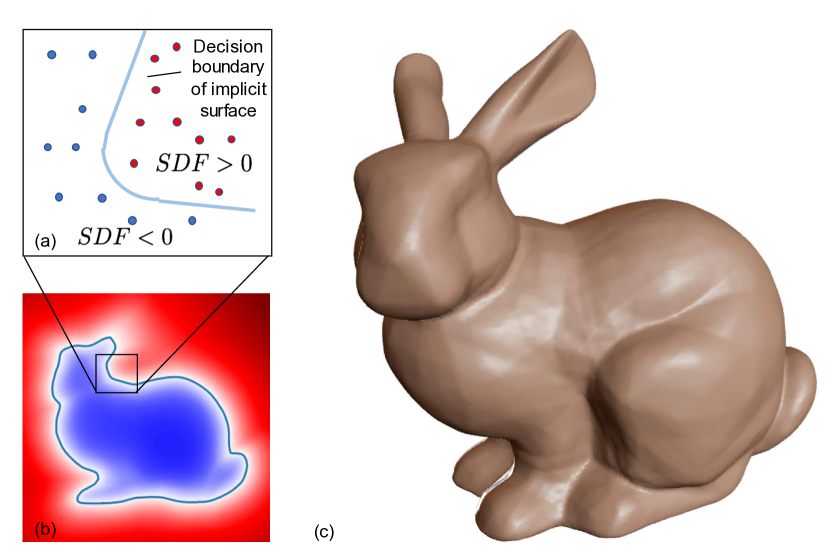
\includegraphics[width=0.6\textwidth]{sdf.png}}
        \caption{(a) depiction of the underlying implicit surface $\text{SDF} = 0$ trained on sampled points inside ($\text{SDF} < 0$) and outside ($\text{SDF} > 0$) the surface, 
        (b) 2D cross-section of the signed distance field, (c) rendered 3D surface recovered from $\text{SDF} = 0$. \cite{deepsdf}}
        \label{fig:nerf}
    \end{figure}

    \newpage
    \textbf{Occupancy Networks} learn a function that maps 3D points to occupancy probability, effectively encoding which parts of space are free or occupied.

    \newpage
    \subsection{Depth Estimation Networks}
    
    Depth estimation is a fundamental component of many SLAM systems, providing crucial 3D structure information from 2D images. Traditional approaches rely on multiple views (stereo or structure from motion) with explicit 
    geometric constraints. Deep learning has transformed this area by enabling accurate depth estimation from limited inputs—even from single images—by leveraging learned priors about the world.
    
    Monocular depth estimation networks address a fundamentally ill-posed problem: recovering scale-ambiguous 3D information from a single 2D projection. These networks succeed by learning statistical relationships between 
    image appearance and geometric structure from large datasets. They effectively encode priors such as:
    
    \begin{itemize}
        \item Typical scales of common objects
        \item Relationship between texture gradients and depth
        \item Perspective effects on parallel lines
        \item Occlusion patterns and their relationship to relative depth
    \end{itemize}
    
    \newpage

    Modern architectures for depth estimation typically use encoder-decoder structures with skip connections, similar to U-Net designs. These networks process images at multiple scales to capture both fine details and broader context.
    For SLAM applications, depth networks are used in several ways:
    
    \textbf{Initialization and Bootstrapping}: Monocular SLAM systems traditionally struggle with initialization and scale estimation. Depth networks provide initial depth maps that establish scale and bootstrap mapping without requiring 
    specific initialization motions.
    
    \textbf{Filling Gaps}: In semi-dense or sparse SLAM systems, learned depth can fill regions where geometric methods fail, particularly in textureless areas or regions with repetitive patterns.
    
    \textbf{Scale Recovery}: Monocular SLAM inherently suffers from scale drift. Depth networks that provide absolute scale estimates can correct this drift throughout operation.
    
    \textbf{Multi-View Consistency}: Modern systems like CNN-SLAM and DeepFactors \cite{deepfactors} use depth predictions as priors in multi-view optimization, combining learning-based initial estimates with geometric refinement.
        
    Self-supervised training has proven particularly valuable, allowing networks to learn from unlabeled video sequences by using photometric consistency loss between frames. This approach enables training on vast amounts of unlabeled 
    data and adaptation to specific environments.
        
    Depth estimation networks have become integral components in state-of-the-art SLAM systems, effectively complementing geometric methods. They are particularly valuable in challenging scenarios such as dynamic scenes, textureless regions, 
    and monocular setups where traditional approaches struggle. As these networks continue to improve in accuracy, efficiency, and generalization capability, their role in SLAM systems is likely to expand further.

    \section{Computer Vision Advancements in SLAM}

    While deep learning has transformed many aspects of SLAM, computer vision continues to drive innovation through specialized techniques that enhance robustness, understanding, and adaptability. These advances focus on solving specific 
    challenges within the SLAM pipeline rather than replacing entire systems.
    
    \subsection{Visual Odometry and Place Recognition}
    
    Visual odometry (VO) estimates camera motion between consecutive frames, forming the backbone of many SLAM systems. Traditional VO approaches rely on geometric constraints and feature matching but struggle in challenging conditions. 
    Recent computer vision advances have significantly improved VO robustness and accuracy.
    

        \begin{figure}[h!]
        \vspace{0.5cm}
        \centering
        \makebox[\textwidth][c]{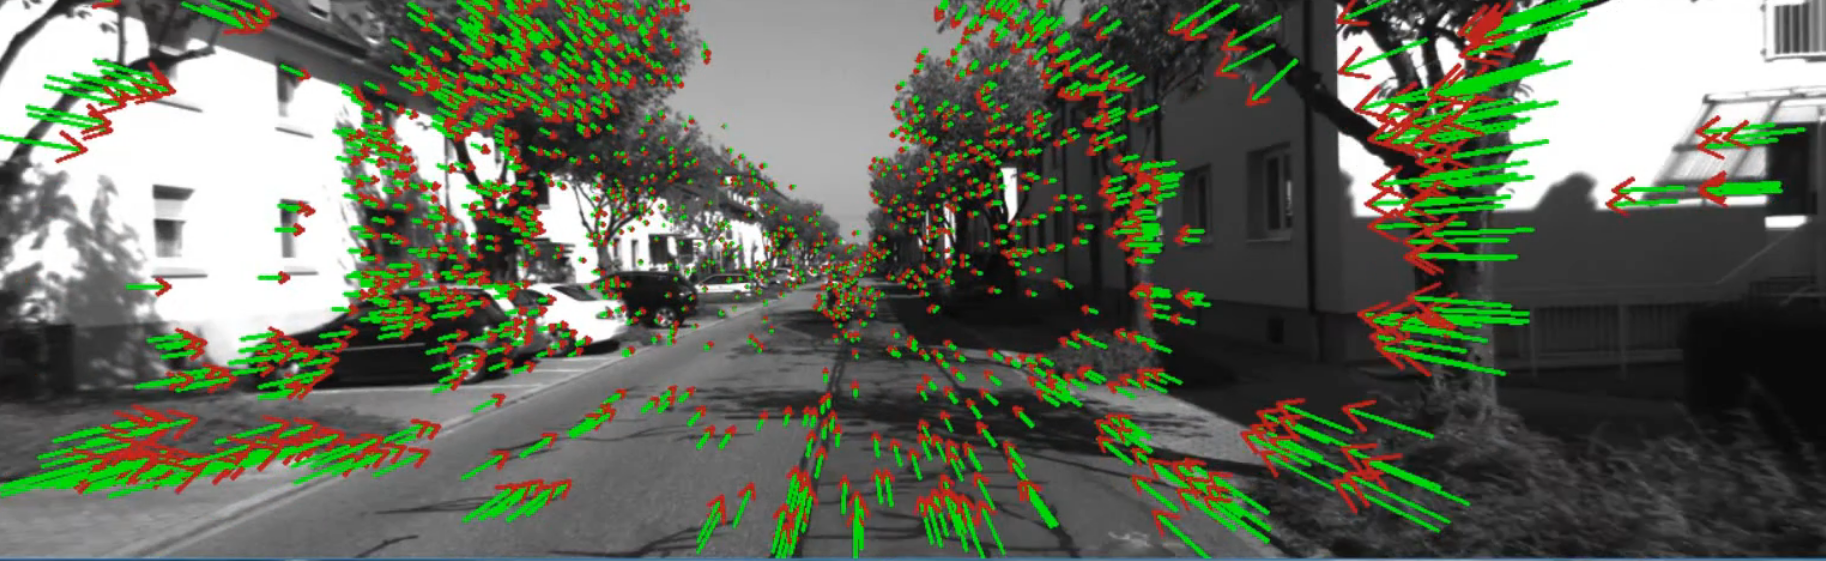
\includegraphics[width=1.0\textwidth]{vis_odometry.png}}
        \caption{Optical flow visualization in a residential street scene showing tracked feature points with motion vectors (green lines)}
        \label{fig:vis_odometry}
    \end{figure}

    \newpage
    \textbf{Learning-Enhanced Visual Odometry} maintains the core geometric principles while using learning for components that benefit most from data-driven approaches:
    
    \begin{itemize}
        \item \textbf{Flow-based Methods} estimate dense optical flow using CNNs and derive camera motion through robust estimation techniques
        \item \textbf{Outlier Rejection Networks} learn to identify unreliable matches that might violate geometric assumptions
        \item \textbf{Confidence Estimation} predicts the reliability of motion estimates, enabling adaptive weighting or fallback strategies
    \end{itemize}
    
    These hybrid approaches maintain the interpretability and geometric correctness of traditional VO while gaining robustness from learning-based components.
    
    \textbf{Place Recognition}, or loop closure detection, has seen transformative improvements through visual embedding techniques. Modern approaches typically follow a retrieval-based paradigm:
    
    \begin{itemize}
        \item \textbf{Image Embedding Networks} map images to compact feature vectors where similar places have similar embeddings regardless of viewpoint or conditions
        \item \textbf{Attention Mechanisms} focus on distinctive environmental elements while ignoring transient objects or lighting variations
        \item \textbf{Sequential Matching} leverages temporal consistency across multiple frames to reduce false positives
    \end{itemize}
        
    The integration of improved VO and place recognition creates SLAM systems that maintain reliable tracking while effectively detecting loops, even in previously challenging environments. 
    This combination addresses the fundamental tension in SLAM between local consistency (through accurate VO) and global consistency (through reliable loop closure).
    
    \subsection{Semantic SLAM}
    Semantic SLAM represents a fundamental paradigm shift from purely geometric reconstruction to scene understanding. By recognizing objects and structures, these systems create maps that capture both spatial layout and semantic meaning.
    Core components include:
    \textbf{Semantic Segmentation} networks (U-Net \cite{u-netformer}, DeepLabv3 \cite{deeplabv3}) classify each pixel in input images into meaningful categories like walls, floors, furniture, and objects.
    \textbf{Object Detection Systems} like Mask R-CNN \cite{mask_r-cnn} identify specific object instances with their boundaries and classes, providing rich information for higher-level mapping.

    \begin{figure}[h!]
        \vspace{0.5cm}
        \centering
        \makebox[\textwidth][c]{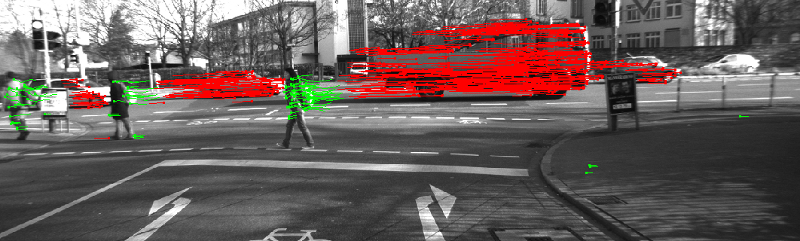
\includegraphics[width=1\textwidth]{visual_odometry.jpg}}
        \caption{Semantic motion segmentation in visual SLAM showing dynamic objects (pedestrians in green, vehicles in red) distinguished from the static environment (grayscale background) through combined visual odometry and object detection, 
        enabling robust localization in urban environments with multiple moving elements. \cite{geiger_lib}}
        \label{fig:visual_odometry}
    \end{figure}

    \newpage
    Semantic mapping approaches integrate this understanding with geometric reconstruction through:
    \begin{itemize}
    \item \textbf{Voxel-Based Fusion} - combining depth and semantic labels in volumetric representations
    \item \textbf{Object-Level Mapping} - using detected objects as primitives instead of points or surfaces
    \item \textbf{Hierarchical Representations} - organizing maps into meaningful layers from geometry to semantics
    \end{itemize}
    This semantic integration provides several crucial benefits: improved data association through object recognition; richer scene understanding for navigation, effective dynamic object handling, more compact map representations, and robust loop closure 
    based on landmark recognition despite appearance changes.
    Object-SLAM exemplifies this evolution by making objects the primary mapping elements. The environment becomes a collection of recognized objects with poses and shapes, often using category-level priors from datasets like ShapeNet \cite{shapenet}. 
    This approach enables meaningful interaction in applications where understanding what objects are and their function is as important as knowing their position.

    \newpage
    \subsection{Dynamic Environment Handling}
    Traditional SLAM systems assume static environments, where sensor reading changes reflect only camera motion. This assumption breaks down in real-world settings with moving objects and changing conditions. Modern approaches address this limitation 
    through several techniques:
    \textbf{Motion Segmentation} identifies moving elements by:
    \begin{itemize}
    \item Detecting geometric inconsistencies in feature tracks or depth measurements
    \item Analyzing optical flow patterns to identify independent motion
    \item Using deep networks specifically trained to segment dynamic objects
    \end{itemize}
    \textbf{Object-Level Dynamics Modeling} goes beyond simple segmentation to track and predict the motion of identified objects. Rather than simply removing dynamic elements, these approaches create trajectory models of moving objects and 
    integrate them into the environmental representation.
    
    \textbf{Long-Term Mapping} addresses environments that change over time, from seasonal variations to rearranged furniture. These methods implement strategies for map management, change detection, and experience-based navigation that maintains 
    different representations of the same location under varying conditions.
    
    \newpage
    \section{Current Research and Applications}

    \subsection{Self-Supervised and Few-Shot Learning}
    
    Recent SLAM research has increasingly focused on reducing dependency on labeled data through self-supervised learning. These approaches leverage inherent geometric and temporal
    consistency in visual data as supervision signals, enabling models to learn without human annotation.
    
    Self-supervised depth estimation trains networks using photometric consistency between multiple views, essentially using the SLAM problem itself as supervision. By warping images based on 
    predicted depth and camera motion, networks learn to minimize reconstruction error without ground truth depth.
    
    Few-shot adaptation tackles the domain gap between training and deployment environments. Rather than requiring complete retraining, these methods adapt pre-trained networks to new environments with minimal data:
    
    \begin{itemize}
        \item Meta-learning approaches learn initial weights that can quickly adapt to new scenarios
        \item Domain adaptation techniques explicitly address shifts in visual appearance
        \item Continual learning methods gradually update models during operation
    \end{itemize}
    
    These advances are making SLAM systems more adaptable and practical for real-world deployment where collecting large labeled datasets for every environment is infeasible.
    
    \newpage
    \subsection{Real-World Applications}
    
    SLAM technologies have matured beyond research labs to power a diverse range of applications:
    
    \textbf{Autonomous Vehicles} use SLAM for localization relative to high-definition maps and real-time obstacle detection. Companies like Waymo, Tesla, and Cruise integrate visual-inertial SLAM with other sensing modalities to create robust navigation systems.
    
    \textbf{Augmented Reality} platforms including Apple's ARKit, Google's ARCore, and Microsoft's HoloLens rely on visual SLAM to track device motion and anchor virtual content in the physical world. These systems must operate on mobile devices with limited computational resources.
    
    \textbf{Service Robotics} applications including vacuum cleaners, delivery robots, and healthcare assistants use SLAM for navigation in homes, hospitals, and offices. These systems prioritize reliability and safety when operating around humans.
    
    \textbf{Industrial Automation} employs SLAM for autonomous forklifts, inventory management, and inspection robots in warehouses and manufacturing facilities. These applications often require operation in challenging environments with reflective surfaces and repetitive structures.
        
    \subsection{Challenges and Future Directions}
    
    Despite impressive progress, several significant challenges remain:
    
    \textbf{Robustness in Extreme Conditions} remains a frontier, particularly in environments with challenging lighting (very bright, very dark, quickly changing), unusual motion patterns, or highly dynamic elements. Future systems will likely integrate multiple sensing modalities and learning-based approaches to handle these edge cases.
    
    \textbf{Resource Constraints} pose limitations for SLAM on embedded platforms like drones, mobile robots, and AR devices. Research on model compression, hardware-aware algorithms, and specialized architectures aims to deliver high-performance SLAM with limited computational resources.
    
    \textbf{Long-term Operation} challenges include drift accumulation, changing environments, and computational resource management over extended periods. Future systems will need better approaches to map maintenance, forgetting irrelevant information, and prioritizing computational effort.
    
    Promising future directions include:
    
    \begin{itemize}
        \item \textbf{Multi-agent Collaborative SLAM} - distributed mapping across multiple robots with information sharing
        \item \textbf{SLAM-aware Planning} - tighter integration between perception and planning systems
        \item \textbf{Foundation Model Integration} - leveraging large pre-trained models for better scene understanding and generalization
    \end{itemize}
    
    As SLAM systems continue to evolve, they will increasingly focus not just on "where am I and what does the world look like?" but on "what can I do in this environment?" This shift toward task-oriented spatial intelligence represents the next frontier in robot perception.

    
    \newpage
    \printbibliography[title={References}]
\end{document}